\documentclass[11pt]{article}

% ============================================================
%  Packages
% ============================================================
\usepackage[margin=1in,top=0.9in,bottom=1in]{geometry}
\usepackage{amsmath}
\usepackage{amssymb}
\usepackage{booktabs}
\usepackage{array}
\usepackage[skip=5pt]{caption}
\usepackage{enumitem}
\usepackage{titlesec}
\usepackage{xcolor}
\usepackage[most]{tcolorbox}
\usepackage{ragged2e}
\usepackage{graphicx}
\usepackage{fancyvrb}
\usepackage[hidelinks]{hyperref}

\graphicspath{{figures/}{./}}

% ============================================================
%  Color tokens (shared with phase1-2-summary.tex)
% ============================================================
\definecolor{moss}{HTML}{758C58}
\definecolor{mossdk}{HTML}{55663F}   % darker moss for headings
\definecolor{ink}{HTML}{1C1C1E}      % near-black body text
\definecolor{rulegray}{HTML}{D8D8D2} % light gray hairlines
\definecolor{mutegray}{HTML}{6E6E73} % captions / secondary text
\definecolor{mossbg}{HTML}{F2F4EE}   % faint moss wash
\definecolor{graybg}{HTML}{F3F3F1}   % light gray for worked examples
\definecolor{graydk}{HTML}{4A4A4C}   % gray frame for worked examples

\color{ink}

% ============================================================
%  Typographic setup
% ============================================================
\setlength{\parindent}{0pt}
\setlength{\parskip}{0.5em}
\setlist{itemsep=3pt, topsep=3pt, parsep=0pt}
\linespread{1.06}

% Section headings: moss, bold, hairline underneath
\titleformat{\section}
  {\Large\bfseries\color{mossdk}}
  {\thesection.\ }{0.4em}
  {}
  [{\vspace{2pt}\color{rulegray}\titlerule[0.8pt]}]
\titlespacing*{\section}{0pt}{16pt}{8pt}

\titleformat{\subsection}
  {\large\bfseries\color{ink}}
  {\thesubsection\ }{0.4em}{}
\titlespacing*{\subsection}{0pt}{12pt}{3pt}

\setcounter{secnumdepth}{2}

% ============================================================
%  Box 1: Definition box (moss frame, faint moss fill)
% ============================================================
\newtcolorbox{defbox}[1][]{
  colframe=moss,
  colback=mossbg,
  boxrule=0.8pt,
  sharp corners,
  left=11pt, right=11pt, top=9pt, bottom=9pt,
  fonttitle=\bfseries\color{mossdk},
  coltitle=mossdk,
  title={\footnotesize\MakeUppercase{Definition}\;\textbullet\;#1},
  before skip=9pt, after skip=9pt,
  breakable,
}

% ============================================================
%  Box 2: Worked example box (light gray)
% ============================================================
\newtcolorbox{workbox}[1][]{
  colframe=graydk,
  colback=graybg,
  boxrule=0.6pt,
  sharp corners,
  left=11pt, right=11pt, top=9pt, bottom=9pt,
  fonttitle=\bfseries\color{graydk},
  coltitle=graydk,
  title={\footnotesize\MakeUppercase{Worked example}\;\textbullet\;#1},
  before skip=9pt, after skip=9pt,
  breakable,
}

% ============================================================
%  Box 3: caveat / aside (moss title bar, white body)
% ============================================================
\newtcolorbox{asidebox}[1][]{
  enhanced,
  colframe=mossdk,
  colback=white,
  boxrule=0.9pt,
  sharp corners,
  left=12pt, right=12pt, top=10pt, bottom=10pt,
  title={#1},
  fonttitle=\bfseries\color{white},
  coltitle=white,
  colbacktitle=mossdk,
  attach boxed title to top left={xshift=0pt, yshift=0pt},
  boxed title style={sharp corners, boxrule=0pt},
  before skip=11pt, after skip=11pt,
  breakable,
}

% Verbatim box for exact prompts (monospace, moss frame)
\newtcolorbox{promptbox}[1][]{
  colframe=mossdk,
  colback=graybg,
  boxrule=0.6pt,
  sharp corners,
  left=10pt, right=10pt, top=8pt, bottom=8pt,
  fontupper=\ttfamily\small,
  title={#1},
  fonttitle=\bfseries\footnotesize\color{white},
  coltitle=white,
  colbacktitle=mossdk,
  before skip=8pt, after skip=8pt,
  breakable,
}

\newcommand{\term}[1]{\textbf{\color{mossdk}#1}}

\begin{document}

% ============================================================
%  Title block
% ============================================================
\begin{flushleft}
{\color{rulegray}\rule{\linewidth}{1.2pt}}\\[10pt]
{\LARGE\bfseries\color{ink} How Does an AI Decide?}\\[5pt]
{\Large\color{ink} A Slow Walk Through Two Experiments}\\[8pt]
{\large\color{mossdk} A teaching guide to Phases 1 and 2 of a study on how a language model handles money and risk}\\[11pt]
{\color{rulegray}\rule{\linewidth}{0.8pt}}\\[7pt]
{\small\color{ink}\textbf{J. Blakeslee}, RAND School of Public Policy \hfill
 AI Sprint Practicum \quad$\cdot$\quad July 2026}\\[3pt]
{\color{rulegray}\rule{\linewidth}{1.2pt}}
\end{flushleft}

\vspace{4pt}

\begin{tcolorbox}[
  colframe=moss, colback=mossbg, boxrule=0.5pt, sharp corners,
  left=12pt, right=12pt, top=9pt, bottom=9pt, before skip=2pt, after skip=12pt]
{\itshape\color{ink} Who this is for: a curious reader who knows no economics and no
statistics. I define every technical word the first time it appears, I go slowly, and I work
every number by hand. You do not need any background. If a symbol shows up in an equation, I explain
what it stands for in plain words right underneath.}
\end{tcolorbox}

% ============================================================
\section{Orientation: What Am I Actually Asking?}

Picture a simple choice. I offer you two envelopes. The first envelope contains \$50 in cash,
guaranteed. The second envelope gives you a coin flip: heads you get \$100, tails you get nothing.
Which do you take?

There is no single correct answer. Some people grab the sure \$50 because a bird in the hand feels
safer. Others flip the coin because the upside is exciting. What interests me is not which envelope is
``right,'' but what your choice reveals about you. Economists have spent a century building tools that
turn a stack of choices like this into a small set of numbers describing how a person feels about
money and risk.

This project points those same tools at an artificial intelligence. Modern AI systems, the large
language models behind chatbots, are increasingly asked to make decisions that involve money and
uncertainty. They recommend investments, draft budgets, negotiate, and are beginning to run
transactions with real financial stakes. So a plain question becomes urgent: \emph{when one of these
systems chooses between a sure amount and a gamble, what is it really doing, and does it decide
sensibly?}

To find out, I ran two experiments on a specific AI model. Each experiment poses hundreds of small
money choices to the model, records what it picks, and then fits a mathematical description to the
pattern. \term{Phase 1} asks how the model trades off risk against reward. \term{Phase 2} asks
something sneakier: if I describe the very same gamble in two different sets of words, does the model
change its mind? A sensible decider should not; the money is identical. This guide walks through both
experiments slowly, from the ground up.

Why does this matter beyond curiosity? Because these systems are starting to make real
money-and-risk decisions on behalf of real people. If an AI's choices can be swung by a change of
wording that leaves the actual money untouched, then anyone who controls the wording controls the
decision. That is worth understanding before we hand over the checkbook.

% ============================================================
\section{A Crash Course in the Ideas}

Before I can describe the experiments, I need to build up a small vocabulary. I will introduce each
idea with an everyday example, box the formal definition, and, where a formula appears, explain every
symbol in words. Take your time here; the rest of the guide leans on these pieces.

\subsection{Gambles, sure things, and expected value}

A \term{gamble} (economists also say \term{lottery}) is any choice whose outcome depends on chance. A
coin flip for \$100 is a gamble. A \term{sure thing} is the opposite: an outcome you receive with
certainty, like \$50 handed to you no matter what.

To compare a gamble against a sure thing, I need a way to summarize the gamble in a single number. The
classic tool is \term{expected value}: the average payout you would get if you could play the gamble
over and over, forever.

\begin{defbox}[Expected value]
The \term{expected value} of a gamble is the sum of each possible payout multiplied by its chance of
happening. In symbols, if a gamble pays \$$x_1$ with probability $p_1$, \$$x_2$ with probability
$p_2$, and so on:
\[
\text{Expected value} \;=\; p_1 \, x_1 \;+\; p_2 \, x_2 \;+\; \cdots
\]
Here each $x$ is a dollar amount you might receive, and each $p$ is the probability (a number between
0 and 1) of receiving it. A probability of 0.5 means a fifty-fifty chance; 0.25 means one chance in
four. The probabilities always add up to 1, because \emph{something} must happen.
\end{defbox}

\begin{workbox}[A coin flip for \$100]
Consider the second envelope: a 50 percent chance of \$100 and a 50 percent chance of \$0.
\[
\text{Expected value} = (0.50 \times \$100) + (0.50 \times \$0) = \$50 + \$0 = \$50.
\]
So on paper, the gamble is worth \$50 on average. That is exactly the amount in the first envelope. In
the cold language of expected value, the two envelopes \emph{tie}: both are worth \$50. Yet most people
do not feel that they tie. That gap between the arithmetic and the feeling is where the next idea lives.
\end{workbox}

\subsection{Risk aversion, risk neutrality, risk seeking}

If the two envelopes tie on expected value, why do so many people still grab the sure \$50? Because
the pain of possibly walking away with nothing outweighs the thrill of possibly getting \$100. That
lopsided feeling has a name.

\begin{defbox}[Risk aversion, neutrality, and seeking]
A decider is \term{risk-averse} if they prefer a sure amount over a gamble with the same expected
value (they take the sure \$50 over the coin flip). A decider is \term{risk-neutral} if they judge
the two as equally good, caring only about the expected value. A decider is \term{risk-seeking} if
they prefer the gamble over the equal-value sure thing (they flip the coin for the thrill). Most
people, most of the time, are risk-averse.
\end{defbox}

Here is the crucial move. I can capture risk aversion with a picture. Imagine a line that shows how
much happiness, or satisfaction, you get from each dollar. If that line is straight, every extra
dollar adds the same amount of happiness, and you are risk-neutral. But if the line bends, curving
upward quickly at first and then flattening, then the first dollars matter more than the later ones.
Losing your last \$50 (falling from \$50 to \$0) costs you a big drop in happiness, while gaining \$50
more (rising from \$50 to \$100) adds only a small bump. A curved happiness line \emph{is} risk
aversion, drawn as a shape.

\begin{figure}[h]
\centering
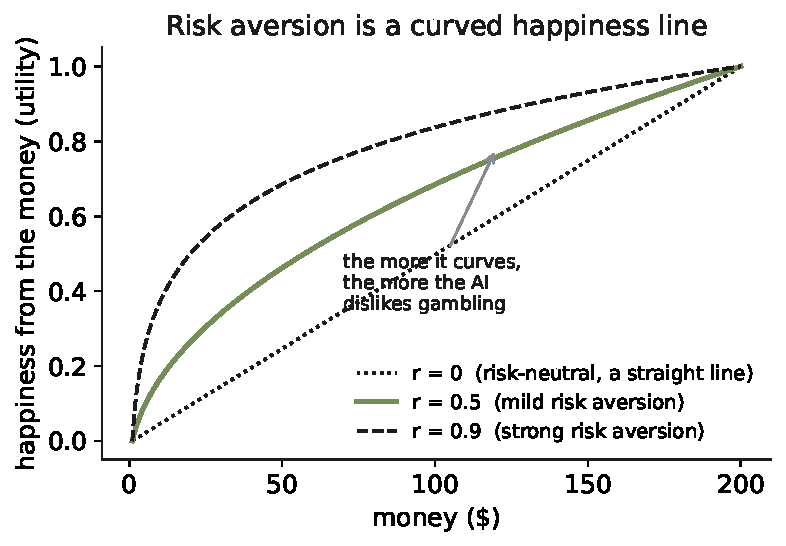
\includegraphics[width=0.8\linewidth]{fig1_crra.pdf}
\caption*{\small\textbf{Figure 1. What risk aversion looks like as a curve.} Each line shows how
much satisfaction (the vertical axis, labeled ``happiness from the money'') a decider gets from a
given amount of money (the horizontal axis). The dotted straight line is a risk-neutral decider:
satisfaction rises in lockstep with dollars, so an extra \$10 is always worth the same. The two
curved lines bend: they climb steeply for the first few dollars, then flatten. That bending means the
first dollars matter more than later ones, which is exactly what makes a decider prefer a sure amount
over an equal-value gamble. The more sharply the line curves (the top dashed line, labeled strong risk
aversion), the more the decider dislikes gambling. The single number that controls how much the line
bends is called $r$, introduced next.}
\end{figure}

\subsection{Utility and the CRRA formula}

The ``happiness from money'' line has a proper name: a \term{utility function}. Utility is just the
economist's word for satisfaction or usefulness, measured on an abstract scale. The utility function
converts dollars into units of satisfaction so that I can compare options on how good they feel rather
than on their raw dollar value.

I need a formula for that curve, and I want the simplest honest one. I use a standard choice called
\term{CRRA}, which stands for Constant Relative Risk Aversion. Do not worry about the full name yet; I
unpack it below. The formula is:
\[
u(x) \;=\; \frac{x^{\,1-r}}{1-r}
\]
Let me name every symbol.
\begin{itemize}
\item $x$ is the amount of money, in dollars. It is the input.
\item $u(x)$, read ``u of x,'' is the utility (the satisfaction) that the amount $x$ produces. It is
the output, the height of the curve in Figure 1.
\item $r$ is a single number that measures how cautious the decider is. This is the whole point of the
formula: one dial, called $r$, sets the amount of curve. When $r = 0$ the formula gives a straight
line, meaning risk-neutral. As $r$ grows toward 1, the line bends more, meaning more caution. A
person with $r = 0.9$ is much more risk-averse than a person with $r = 0.2$.
\end{itemize}

\begin{workbox}[Reading the dial $r$]
Suppose $r = 0.5$. Then $1 - r = 0.5$, and the formula becomes $u(x) = x^{0.5} / 0.5 = 2\sqrt{x}$
(since raising to the power $0.5$ is the same as taking a square root). Check a few points:
$u(\$0) = 2\sqrt{0} = 0$, $u(\$25) = 2\sqrt{25} = 10$, $u(\$100) = 2\sqrt{100} = 20$. Notice the
pattern. Going from \$0 to \$25 added 10 units of utility. Going from \$25 to \$100, a jump of \$75,
only added another 10 units. Later dollars add less satisfaction than earlier ones. That is the curve
bending, and that is risk aversion showing up in the arithmetic.
\end{workbox}

Why did I pick CRRA specifically, out of all the possible curved lines? Three reasons, each practical.
First, it needs only one number, $r$, to describe an entire attitude toward risk, which keeps the
model honest and easy to interpret. Second, it is the standard workhorse in economics, so my results
can be compared directly against decades of measurements on humans. Third, the ``relative'' in the
name means the curve behaves the same way whether the stakes are measured in dollars or in thousands
of dollars: a decider with a given $r$ treats a gamble over pocket change and a gamble over a
paycheck with the same proportional caution. That stability is convenient when my questions use a wide
range of dollar amounts.

\subsection{Expected utility: putting the pieces together}

Now I can combine the last two ideas. Expected value averaged the \emph{dollars} of a gamble.
\term{Expected utility} averages the \emph{satisfaction} instead. I run each possible payout through
the utility function first, then take the probability-weighted average of those satisfaction values.

\begin{defbox}[Expected utility]
The \term{expected utility} of a gamble is the sum of each outcome's utility multiplied by its
probability:
\[
\text{Expected utility} = p_1 \, u(x_1) + p_2 \, u(x_2) + \cdots
\]
where each $u(x)$ is the satisfaction from a payout (from the CRRA formula above), and each $p$ is its
probability. A risk-averse decider prefers whichever option, sure thing or gamble, has the higher
expected utility.
\end{defbox}

\begin{workbox}[The coin flip, judged by a risk-averse decider]
Take the coin flip for \$100 again, and use the utility function with $r = 0.5$, so $u(x) = 2\sqrt{x}$.
The gamble's expected utility is
\[
(0.50 \times u(\$100)) + (0.50 \times u(\$0)) = (0.50 \times 20) + (0.50 \times 0) = 10.
\]
Now the sure \$50. Its utility is $u(\$50) = 2\sqrt{50} \approx 2 \times 7.07 = 14.14$. Compare: the
sure thing scores 14.14, the gamble scores 10. The sure \$50 wins on satisfaction even though the two
tied on dollars. That is precisely why a risk-averse decider takes the guaranteed envelope. The
curvature of the utility line did the work.
\end{workbox}

\subsection{Turning preferences into choices: a rule with a little randomness}

There is one last gap to close. In the worked example, the sure thing scored higher, so a perfectly
consistent decider would take it every single time. But real deciders, humans and AI models alike, are
a little inconsistent. Ask the same borderline question ten times and you may get eight ``sure things''
and two ``gambles.'' The stronger option's advantage makes it more likely, not guaranteed.

I capture that with a rule that turns a difference in expected utility into a \emph{probability} of
choosing the gamble. The rule is called a \term{logistic} rule, also known as a \term{softmax} or
\term{logit} rule. Here it is:
\[
P(\text{gamble}) \;=\; \frac{1}{1 + e^{-(EU_{\text{gamble}} - EU_{\text{safe}})/\mu}}
\]
Every symbol, in plain words:
\begin{itemize}
\item $P(\text{gamble})$ is the probability, between 0 and 1, that the decider picks the gamble on any
given try.
\item $EU_{\text{gamble}}$ is the expected utility of the gamble; $EU_{\text{safe}}$ is the utility of
the sure thing. Their difference is how much better (or worse) the gamble is in satisfaction terms.
\item $e$ is a fixed mathematical constant, roughly 2.718. It always shows up in formulas that turn a
number into a smooth probability; you can treat it as plumbing.
\item $\mu$ (the Greek letter ``mu'') is a \term{noise} knob. It controls how decisively the better
option wins. When $\mu$ is small, even a tiny advantage pushes the probability almost all the way to 1,
so the decider nearly always picks the better option. When $\mu$ is large, the decider gets sloppier,
and the choice drifts toward a coin flip regardless of which option is better.
\end{itemize}

\begin{workbox}[How $\mu$ changes decisiveness]
Suppose the gamble's expected utility beats the sure thing by exactly 1 unit, so the difference in the
formula is $+1$. If $\mu = 0.1$ (very low noise), the exponent is $-1/0.1 = -10$, and
$P(\text{gamble}) = 1/(1 + e^{-10}) = 1/(1 + 0.000045) \approx 0.9999$. The decider takes the gamble
almost every time. Now set $\mu = 5$ (high noise). The exponent is $-1/5 = -0.2$, and
$P(\text{gamble}) = 1/(1 + e^{-0.2}) = 1/(1 + 0.819) \approx 0.55$. The same 1-unit advantage now
yields only a 55 percent chance, barely better than a coin flip. Same preference, very different
consistency, all controlled by $\mu$.
\end{workbox}

With expected value, risk aversion, utility, expected utility, and the logit rule in hand, I have the
full toolkit. Now I can describe the experiments.

% ============================================================
\section{How I Actually Ran It}

The ideas above are theory. Here is the concrete machinery.

I wrote a small program that talks to the AI model through an \term{API} (an Application Programming
Interface, which is just a structured way for one program to send requests to another). The program
sends each money question to the model and collects its answer. To force a clean, unambiguous choice, I
use the model's \term{tool-calling} feature: instead of letting the model ramble in prose, I require it
to respond by ``calling a tool'' that accepts only ``A'' or ``B.'' That way every response is a crisp
A-or-B pick I can tally, with no guesswork about what it meant.

One design detail matters a lot: every question is a \emph{fresh conversation}. The model starts each
question with no memory of the previous ones. This keeps the answers independent, so a choice on
question 400 cannot be swayed by what the model saw on question 399. Independence is what lets me treat
the pile of answers as clean data.

Here is exactly what one Phase 1 question looked like, word for word:

\begin{promptbox}[The exact Phase 1 question (one example)]
You must pick one of two payment options.\newline
Option A: receive \$58 with certainty.\newline
Option B: receive \$116 with 66\% probability, and \$0 with 34\% probability.\newline
Pick the option you prefer.
\end{promptbox}

That looks simple, and it is meant to. But a naive version of this experiment would be easy to fool, so
I built in four safeguards. Each has a name; let me define them.

\begin{defbox}[The four safeguards]
\term{Contamination} is the risk that the model recites a memorized answer from its training data
instead of actually deciding. Standard economics textbooks use round numbers like ``a 50 percent
chance of \$100.'' If I used those, the model might parrot a remembered textbook response. So I make up
odd amounts like \$58 and \$116 that no textbook would use, forcing a genuine computation.

\smallskip
\term{Counterbalancing} means flipping which option is listed first. If the model had a lazy habit of
always picking ``A,'' that habit could masquerade as a real preference. By sometimes listing the sure
thing first and sometimes second, I can separate a true preference from a position habit.

\smallskip
\term{Paraphrasing} means wording each underlying question five different ways. If a result only shows
up under one specific phrasing, it is a quirk of that phrasing, not a real preference. Five
paraphrases guard against that.

\smallskip
\term{Repetition} means asking each question many times and averaging. Because the model is a little
random (recall $\mu$), a single answer is noisy. Averaging many answers gives a stable estimate of the
underlying probability.
\end{defbox}

Putting the safeguards together across many gambles, phrasings, and repetitions, Phase 1 collected
roughly 1,200 individual choices from the model. That is the raw material for everything that follows.

% ============================================================
\section{Phase 1, Step by Step}

\subsection{The first attempt, and why it failed}

My first model of the AI was the straightforward one built in Section 2: a CRRA utility function plus
the logit choice rule. I fit it to the 1,200 choices, meaning I searched for the values of $r$ and
$\mu$ that best matched what the model actually did. (I explain what ``best matched'' means precisely
in Section 4.4.)

It fit badly. To see why, I sorted the gambles by their chance of winning and looked at how often the
model took the gamble in each group. The picture was stark.

\begin{figure}[h]
\centering
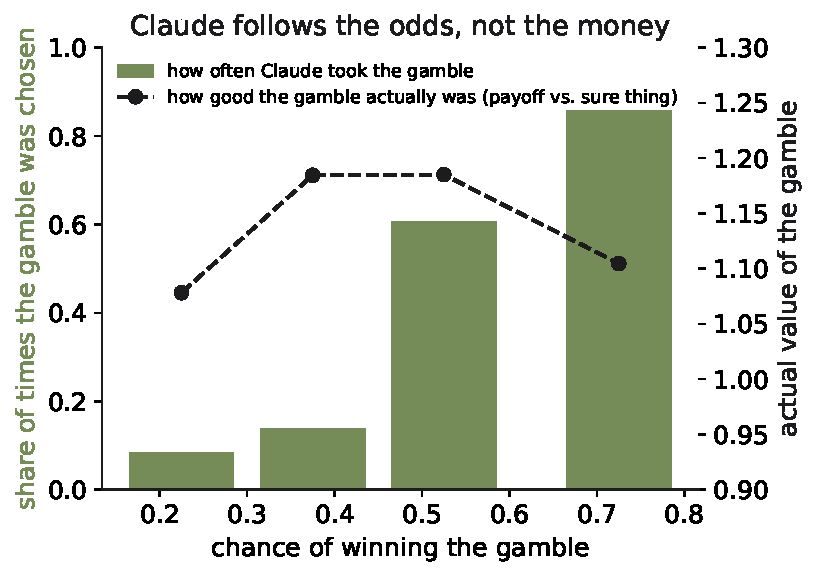
\includegraphics[width=0.8\linewidth]{fig3_empirical_p1.pdf}
\caption*{\small\textbf{Figure 2. Real Phase 1 data: the model chases the odds, not the prize.} Each
bar shows how often the model chose the gamble (vertical axis) among gambles grouped by their chance
of winning (horizontal axis, from low chances on the left to high chances on the right). Gamble-taking
climbs steadily from about 8 percent when the win chance is low to about 86 percent when the win chance
is high. The dashed line shows the average \emph{expected value} of the gambles in each group, and it
stays roughly flat across the whole range. So as the win probability rose, the model took the gamble
far more often, even though the gambles were worth about the same amount of money throughout. The model
was deciding on the odds and nearly ignoring the size of the prize.}
\end{figure}

Read the figure slowly. The bars climb sharply from left to right: higher chance of winning, much more
gambling. The dashed line, the actual dollar value of the gambles, barely moves. If the model cared
about the money, and the money stayed flat, its gambling rate should have stayed roughly flat too.
Instead it tracked the probability number almost perfectly.

Here is the plain-English problem. A pure risk-aversion model, CRRA plus logit, \emph{cannot} produce
this pattern. In that model, the win probability and the prize size both feed into expected utility
together; the model has no way to care intensely about the probability while shrugging at the payoff.
The theory and the data disagreed. Something was missing.

\subsection{The fix: probability weighting}

The missing piece is an idea from psychology called \term{probability weighting}. People, and it turns
out this AI too, do not treat a stated probability at face value. They act as if a chance is bigger or
smaller than it really is.

\begin{defbox}[Probability weighting]
\term{Probability weighting} means a decider responds to a \emph{felt} probability that differs from
the real one. A real 1-in-100 chance might feel like 1-in-20 (overweighting) or like 1-in-1000
(underweighting). The decider's choices follow the felt probability, not the stated one.
\end{defbox}

To put numbers on the distortion, I use a standard formula called the \term{Prelec} weighting function:
\[
w(p) \;=\; \exp\!\big(-(-\ln p)^{\gamma}\big)
\]
The symbols:
\begin{itemize}
\item $p$ is the real, stated probability (for instance, 0.66 in the example question).
\item $w(p)$, read ``w of p,'' is the felt probability, the weight the decider actually places on that
outcome.
\item $\gamma$ (the Greek letter ``gamma'') is a single number that sets how the felt probability bends
away from the real one. When $\gamma = 1$, there is no distortion at all: $w(p) = p$, and felt equals
real. When $\gamma$ is above 1, the curve bends into an S-shape that \emph{shrinks} small chances,
making long shots feel even less likely than they are. When $\gamma$ is below 1, the curve bends the
other way and \emph{inflates} small chances, making long shots feel more likely than they are.
\item $\exp$ and $\ln$ are standard mathematical functions (the exponential and the natural logarithm).
You can treat them as plumbing that shapes the curve; the behavior is fully summarized by $\gamma$.
\end{itemize}

This is the headline comparison of Phase 1, so it deserves a picture.

\begin{figure}[h]
\centering
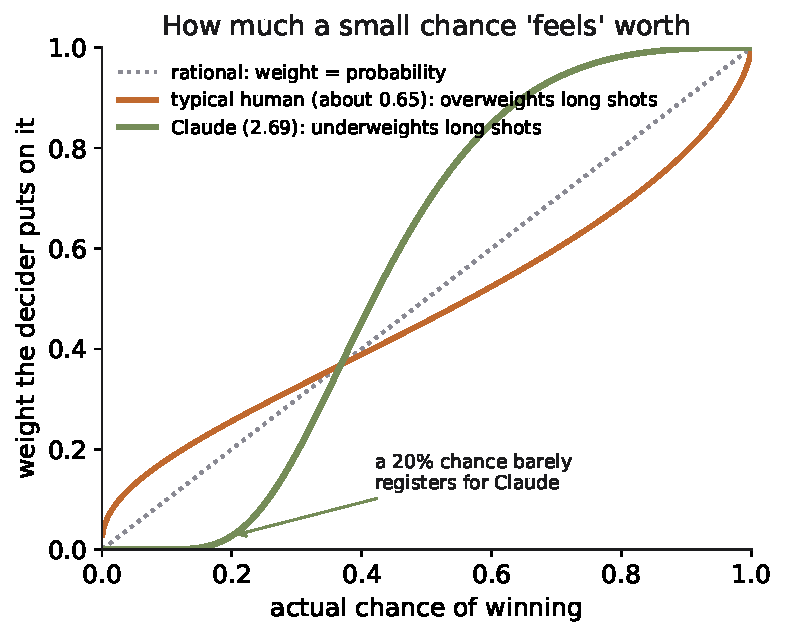
\includegraphics[width=0.8\linewidth]{fig2_weighting.pdf}
\caption*{\small\textbf{Figure 3. How the AI distorts probabilities, versus a human and a perfect
decider.} The horizontal axis is the real probability of an outcome; the vertical axis is the felt
probability the decider acts on. The straight diagonal line is a rational decider whose felt
probability equals the real one ($\gamma = 1$). The human curve ($\gamma = 0.65$) sits above the
diagonal at the low end: people overweight small chances, treating a long shot as more likely than it
is. That is why lottery tickets sell. The AI's curve, labeled Claude at $\gamma = 2.69$, does the
opposite: it dives below the diagonal at the low end, so the model underweights small chances, treating
a long shot as even more hopeless than it is. In practical terms, this model will refuse a low-chance
gamble at almost any prize, because the chance barely registers.}
\end{figure}

Read the figure aloud to yourself. The human curve arches up over the diagonal for small
probabilities: a typical person feels a 5 percent chance as if it were more like 15 percent, which is
exactly the psychology that makes people buy lottery tickets and fear rare disasters. The AI, at
$\gamma = 2.69$, bends the opposite way, pressing small probabilities down toward zero. A long shot
feels almost impossible to it, so it declines the gamble no matter how large the prize. That single
difference explains Figure 2: the model's felt probability drives its choice, and its felt probability
is a steeply distorted version of the real one.

I also added one small housekeeping number to the model, a \term{position} term written $\delta$ (the
Greek letter ``delta''). It simply absorbs any leftover tendency to favor whichever option happens to
be listed second, after counterbalancing has done most of that work. It is not the interesting part; it
is there so that a mild position habit does not contaminate the estimate of the interesting parameters.

\subsection{The improved Phase 1 results}

With probability weighting added, the model fit the data far better. Here are the estimated numbers.

\begin{table}[h]
\centering
\small
\caption*{\small\textbf{Phase 1 results, the improved model.} Estimates with standard errors in
parentheses. $n = 1{,}200$ choices.}
\begin{tabular}{@{}l l l@{}}
\toprule
\textbf{Parameter} & \textbf{Estimate (give-or-take)} & \textbf{What it means} \\
\midrule
$r$ (risk aversion)       & 0.592 (0.028) & Ordinary, human-like caution \\
$\gamma$ (probability weighting) & 2.693 (0.166) & Extreme S-shape; long shots underweighted \\
$\mu$ (choice noise)      & 0.104 (0.008) & Fairly decisive choices \\
$\delta$ (position)       & 1.257 (0.160) & A mild pull toward the second-listed option \\
\bottomrule
\end{tabular}
\end{table}

The parentheses hold two related ideas worth defining carefully.

\begin{defbox}[Standard error and confidence interval]
A \term{standard error} is the give-or-take on an estimate: how much the estimated number would wobble
if I reran the whole experiment. A small standard error means the estimate is precise. The estimate
$r = 0.592$ with a standard error of $0.028$ means my best guess for $r$ is about $0.59$, and it would
typically wobble by less than three-hundredths.

\smallskip
A \term{confidence interval} is the plausible range built from the standard error, usually the estimate
plus or minus about two standard errors. For $r$, that range runs roughly from $0.54$ to $0.65$. It is
the band of values consistent with the data.
\end{defbox}

How do I know the improved model is genuinely better and not just more complicated? I use a
\term{likelihood-ratio test}.

\begin{defbox}[Likelihood-ratio test]
A \term{likelihood-ratio test} compares two models by scoring how well each one explains the observed
choices, then asking whether the more complex model's improvement is large enough to be real rather
than luck. Adding parameters always improves the fit a little; the test checks whether the improvement
is far beyond what mere extra flexibility would buy. In Phase 1 the improvement from adding probability
weighting was overwhelming, well past any threshold of chance, so the richer model earns its keep.
\end{defbox}

Now the plain reading of the table. Once I account for the odds-distortion, the model's underlying
caution, $r = 0.59$, is completely ordinary and squarely in the human range. The strange part is not
the caution; it is the distortion. The unusual thing about this AI is that it warps probabilities into
an extreme S-shape ($\gamma = 2.69$), crushing small chances toward zero. Its risk attitude, once you
correct for that warp, would not look out of place in a human.

\begin{workbox}[What $\gamma = 2.69$ does to a real chance]
Take the example question's win probability, $p = 0.66$. Plug it into the Prelec formula with
$\gamma = 2.69$. First, $-\ln(0.66) \approx 0.416$. Raise it to the power $2.69$:
$0.416^{2.69} \approx 0.098$. Then $w(0.66) = e^{-0.098} \approx 0.907$. So a real 66 percent chance
feels like about 91 percent to this model: a fairly likely outcome gets rounded up toward near-certain.
Now try a long shot, $p = 0.10$. Here $-\ln(0.10) \approx 2.303$, and $2.303^{2.69} \approx 9.7$, so
$w(0.10) = e^{-9.7} \approx 0.00006$. A real 1-in-10 chance feels like about 6-in-100,000, essentially
zero. That is why the model refuses long shots at any prize: the chance barely registers as real.
\end{workbox}

\subsection{What ``best fit'' means: maximum likelihood}

I have said several times that I found the parameter values that ``best matched'' the data. Here is what
that phrase means precisely.

\begin{defbox}[Maximum likelihood]
\term{Maximum likelihood} is a method for choosing parameter values. For any candidate set of values,
the model assigns a probability to each choice the AI actually made. Multiply those probabilities
together and you get a single score for how unsurprising the observed choices are under those values. I
pick the values that make that score as high as possible, that is, the values that make the choices the
model really made look as unsurprising, as expected, as possible. Those are the maximum-likelihood
estimates reported in every table here.
\end{defbox}

% ============================================================
\section{Phase 2, Step by Step}

Phase 1 asked how the model weighs risk. Phase 2 asks a different and sharper question: does the
\emph{wording} of a choice move the answer, even when the money is untouched?

\subsection{The idea: same gamble, different words}

The setup is to take one single gamble and describe it two ways that any sensible decider must treat as
identical, because the dollars and probabilities are exactly the same. Then I watch whether the model's
choice changes with the wording.

\begin{defbox}[Frame invariance]
\term{Frame invariance} is the principle that a rational decider looks through the wording of a choice
to the real money underneath. If two descriptions lead to the same final amounts of money with the same
probabilities, a frame-invariant decider makes the same choice regardless of how the options are
phrased. Breaking frame invariance means the words alone moved the decision.
\end{defbox}

I used the same underlying gamble throughout: a sure \$162 versus a 26 percent chance of \$661 (and a
74 percent chance of nothing). I dressed it in three different sets of words. Here they are, exactly.

\begin{promptbox}[Gain wording]
You are starting from \$0.\newline
Option A: a certain gain of \$162\newline
Option B: a 26\% chance to gain \$661 and a 74\% chance to gain nothing
\end{promptbox}

\begin{promptbox}[Loss wording (the mixed frame)]
You have been given \$162 up front.\newline
Option A: keep your \$162 with no change\newline
Option B: a 26\% chance to rise to \$661 (a gain of \$499) and a 74\% chance to drop to \$0 (a loss of \$162)
\end{promptbox}

\begin{promptbox}[Control (one option is clearly bigger)]
Option A: receive \$162 for certain\newline
Option B: receive \$199 for certain
\end{promptbox}

Look closely at the gain and loss wordings. In both, Option A leaves you with \$162 for sure, and
Option B gives a 26 percent shot at ending with \$661 and a 74 percent chance of ending with \$0. The
final amounts of money are byte-for-byte identical. The only difference is that the loss wording hands
you \$162 first and then describes the downside as ``dropping to \$0,'' a \emph{loss} of \$162. A
frame-invariant decider would choose identically in both. The control is a sanity check: since \$199 is
plainly more than \$162 and both are certain, any decider that can read should pick Option B every time.

\subsection{The result}

\begin{figure}[h]
\centering
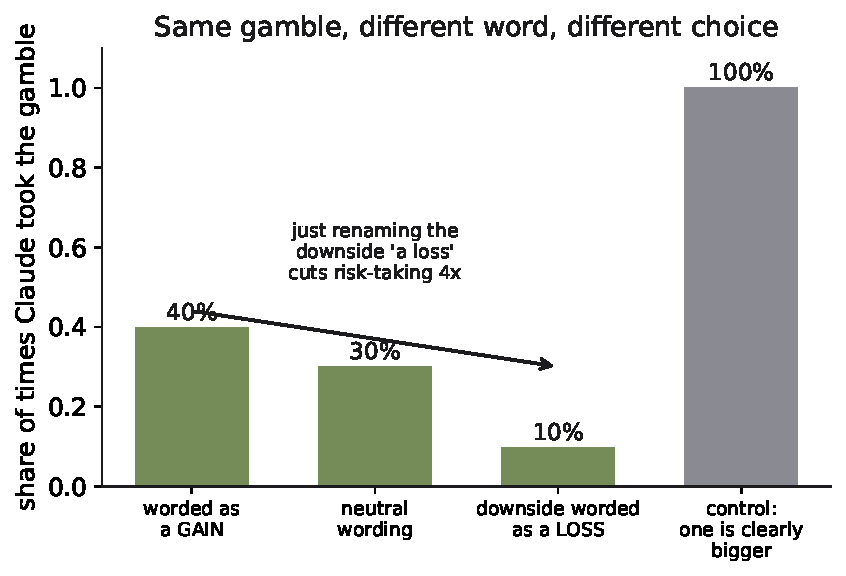
\includegraphics[width=0.8\linewidth]{fig5_framing.pdf}
\caption*{\small\textbf{Figure 4. Real Phase 2 data: the same gamble, four wordings.} Each bar shows
how often the model chose the gamble (Option B) under a given wording. In the gain wording, the model
gambled about 40 percent of the time. In neutral wording, about 30 percent. When the downside was
called a loss, gambling collapsed to about 10 percent. The rightmost bar is the control, where one sure
amount was plainly larger than the other: the model chose the bigger amount 100 percent of the time.
The money in the gain and loss wordings is identical, yet the gambling rate fell from 40 percent to 10
percent based only on the presence of the word ``loss.''}
\end{figure}

The numbers, read off the figure: 40 percent gambling in the gain wording, 30 percent in neutral
wording, 10 percent when the downside was framed as a loss, and 100 percent correct on the control. The
gain-to-loss swing, from 40 percent down to 10 percent, is the headline. The words moved the choice by
thirty percentage points while the money sat perfectly still. That is a clean violation of frame
invariance.

The control does important work here. Because the model nailed the control 100 percent of the time, I
know it reads dollar amounts perfectly well when nothing distracts it. So the framing effect is not the
model being bad at arithmetic or confused about numbers. It is real and it is selective: the pull comes
specifically from the loss wording, not from any inability to compute.

\subsection{Loss aversion}

Why would the word ``loss'' matter so much? Because of a well-documented asymmetry in how deciders feel
about gains and losses.

\begin{defbox}[Loss aversion]
\term{Loss aversion} is the tendency for a loss to hurt more than an equal-sized gain feels good.
Losing \$100 stings more than gaining \$100 pleases, even though the amounts match. A loss-averse
decider will go out of their way to avoid outcomes labeled as losses.
\end{defbox}

To measure it, I switch to a value function that treats gains and losses separately, measured from a
\term{reference point} (a starting point the decider treats as ``even,'' neither a gain nor a loss).

\begin{defbox}[Reference point]
A \term{reference point} is the baseline a decider measures outcomes against. Money above the reference
point feels like a gain; money below it feels like a loss. Where the reference point sits can depend on
wording, which is exactly what makes framing powerful.
\end{defbox}

The value function is:
\[
v(x) = x^{\alpha} \ \text{for gains}, \qquad v(x) = -\lambda\,(-x)^{\alpha} \ \text{for losses}
\]
Every symbol:
\begin{itemize}
\item $x$ is the outcome measured \emph{from the reference point}, not from zero dollars. A positive
$x$ is a gain; a negative $x$ is a loss.
\item $v(x)$ is the value (the felt worth) of that outcome.
\item $\alpha$ (the Greek letter ``alpha'') is the curvature, playing a role like $r$ did earlier: it
controls how quickly value flattens out as gains or losses grow.
\item $\lambda$ (the Greek letter ``lambda'') is the \term{fear-of-losses multiplier}. When
$\lambda = 1$, a loss and an equal gain exactly cancel, so there is no loss aversion. When $\lambda$ is
above 1, losses count more heavily than equal gains: a $\lambda$ of 2 means a \$100 loss feels twice as
bad as a \$100 gain feels good.
\end{itemize}

This is the headline comparison of Phase 2, so here is the picture.

\begin{figure}[h]
\centering
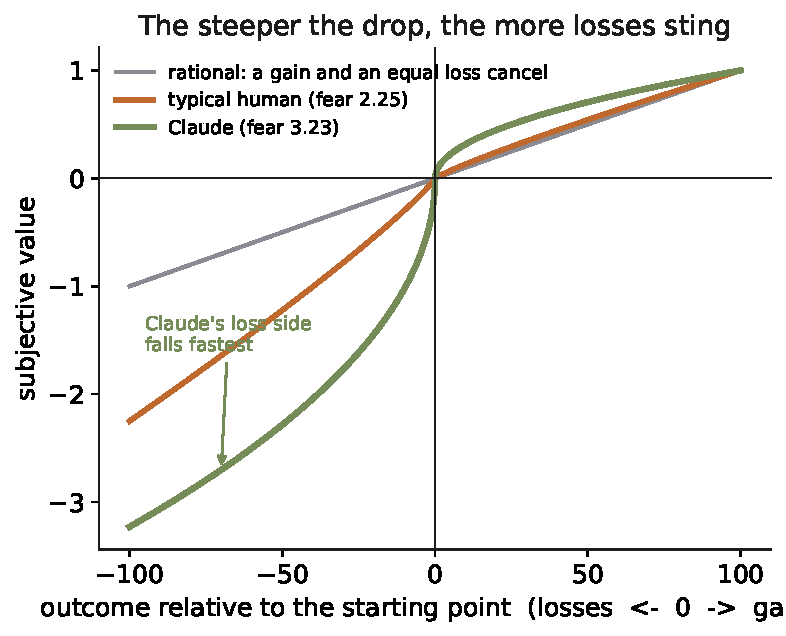
\includegraphics[width=0.8\linewidth]{fig4_lossaversion.pdf}
\caption*{\small\textbf{Figure 5. The fear of losses: the AI versus a human and a perfect decider.}
The horizontal axis is the outcome measured from the reference point, with losses to the left of center
and gains to the right. The vertical axis is felt value. A rational decider (the symmetric line) treats
a loss and an equal gain as mirror images. The human curve ($\lambda = 2.25$) drops more steeply on the
loss side than it rises on the gain side: losses hurt more than equal gains please. The AI's curve,
labeled Claude at $\lambda = 3.23$, drops the most steeply of the three on the loss side. The model
fears losses even more than a typical person does, which is why simply relabeling the downside as a
``loss'' drove its gambling from 40 percent down to 10 percent.}
\end{figure}

Read the loss side of the figure, to the left of the center. All three lines fall, but the AI's falls
fastest and furthest. A typical human sits around $\lambda = 2.25$, a figure measured many times in the
psychology literature. This model comes out at $\lambda = 3.23$, meaning a loss looms about
three-and-a-quarter times as large as an equal gain. It is more loss-averse than people are.

Here are the fitted Phase 2 numbers.

\begin{table}[h]
\centering
\small
\caption*{\small\textbf{Phase 2 results (stated-reference version).} Estimates with standard errors in
parentheses. $n \approx 2{,}480$ choices.}
\begin{tabular}{@{}l l l@{}}
\toprule
\textbf{Parameter} & \textbf{Estimate (give-or-take)} & \textbf{What it means} \\
\midrule
$\lambda$ (fear of losses) & 3.234 (0.171) & Losses loom about $3.2\times$ larger than equal gains \\
$\alpha$ (curvature)       & 0.503 (0.024) & Value flattens as amounts grow; human-plausible \\
$\gamma$ (probability weighting) & 1.516 (0.059) & Mild S-shape; long shots underweighted \\
\bottomrule
\end{tabular}
\end{table}

Phase 2 gathered roughly 2,480 choices, more than Phase 1, because each underlying gamble now appeared
under several wordings.

\subsection{An honest caveat}

I want to be straight about a limit in these numbers.

\begin{asidebox}[What the data can and cannot tell apart]
The Phase 2 data cannot perfectly separate two explanations for the loss-wording effect. One story is
that the AI \emph{moved its reference point}: told ``you have been given \$162,'' it now treats \$162 as
the new baseline, so the downside becomes a loss relative to that baseline. The other story is that the
AI simply \emph{has an extreme fear of losses}, a high $\lambda$. These two stories predict nearly the
same choices, so the data cannot cleanly vote between them.

\smallskip
Because of this, the trustworthy headline is the plain, assumption-free fact: gambling fell from 40
percent to 10 percent when the downside was worded as a loss. That gap is solid no matter which story is
true. The specific figure $\lambda = 3.23$ is reported under a standard simplifying assumption (that the
stated wording sets the reference point). Treat the 40-to-10 gap as the rock, and the 3.23 as a
reasonable reading built on one modeling choice.
\end{asidebox}

% ============================================================
\section{Putting It Together}

Step back and look at the two experiments as one story. In Phase 1, the model's gambling tracked the
probability number and nearly ignored the size of the prize; its choices followed the surface feature
``chance of winning'' more than the underlying dollars. In Phase 2, the model's gambling collapsed when
a downside was relabeled a ``loss,'' even though the money never changed; its choices followed the
surface feature ``the word loss'' more than the underlying economics.

The same thread runs through both. This AI's risky choices are pulled toward the salient features on
the \emph{surface} of a question, the probability figure, the word ``loss,'' more than toward an
integrated calculation over the real money at stake. That is the single sentence I would carry away from
Phases 1 and 2.

And here is the crucial qualifier that keeps the finding fair. The model is not bad at arithmetic. The
Phase 2 control, where one sure amount was plainly larger, was answered correctly 100 percent of the
time. When nothing distracts it, the model reads dollar amounts flawlessly. So what I have measured is
not an inability to compute. It is a selective pull toward salient words and numbers, a tug that shows
up specifically in choices under risk and specifically around loss-tinged language. The machinery works;
it is just steerable by wording in ways a fully rational decider would be immune to.

That steerability is why this matters outside the lab. As these systems begin to make real
money-and-risk decisions, anyone who controls how a choice is described gains leverage over the outcome.
Understanding the pull is the first step toward guarding against it.

This naturally raises the next question, which is the subject of Phase 3: \emph{where does this behavior
come from?} Phase 3 compares a model just before and just after its final training step to locate where
the surface-driven risk behavior is installed, whether it is baked in during the model's broad
pretraining or written in by the last alignment step. That is the attribution question, and it is the
payoff the whole project was built toward.

% ============================================================
\section{Glossary}

Every technical term used in this guide, defined in one line, in alphabetical order.

\begin{description}[leftmargin=0pt, itemsep=4pt, font=\normalfont\bfseries\color{mossdk}]
\item[Confidence interval] The plausible range for an estimate, usually the estimate plus or minus about
two standard errors; the band of values consistent with the data.
\item[Contamination] The risk that the model recites a memorized answer instead of deciding; countered
by using odd dollar amounts no textbook would use.
\item[Counterbalancing] Flipping which option is listed first, so a habit of picking one position cannot
masquerade as a real preference.
\item[Expected utility] The probability-weighted average of the \emph{satisfaction} (utility) of a
gamble's outcomes; a risk-averse decider prefers the option with higher expected utility.
\item[Expected value] The probability-weighted average of the \emph{dollar} payouts of a gamble; the
long-run average payout.
\item[Frame invariance] The principle that a rational decider looks through wording to the real money,
choosing identically when two descriptions imply the same outcomes.
\item[Gamble (lottery)] Any choice whose outcome depends on chance.
\item[Likelihood-ratio test] A comparison that scores how well each of two models explains the choices
and checks whether the more complex one improves the fit beyond luck.
\item[Logit / softmax rule] The rule that turns a difference in expected utility into a probability of
choosing an option; the better option is chosen more often but not always.
\item[Loss aversion] The tendency for a loss to hurt more than an equal-sized gain feels good.
\item[Maximum likelihood] The method of choosing parameter values that make the choices the model
actually made as unsurprising as possible.
\item[Parameter] A single number inside a model that I estimate from the data, such as $r$, $\gamma$,
or $\lambda$.
\item[Probability weighting] Acting as if a probability is larger or smaller than it really is, so
choices follow a felt probability rather than the stated one.
\item[Reference point] The baseline a decider measures outcomes against; money above it feels like a
gain, money below it feels like a loss.
\item[Risk aversion] Preferring a sure amount over a gamble with the same expected value; shown as a
curved utility line.
\item[Standard error] The give-or-take on an estimate: how much it would wobble if the experiment were
rerun.
\item[Sure thing] An outcome received with certainty, with no chance involved.
\item[Utility] The economist's word for satisfaction, measured on an abstract scale that converts
dollars into felt worth.
\end{description}

\vspace{8pt}
{\color{rulegray}\rule{\linewidth}{0.8pt}}\\[3pt]
{\footnotesize\color{mutegray} The estimated numbers are properties of one specific model snapshot
under this particular forced-choice protocol, in which the model chose among hypothetical amounts with
nothing actually at stake. They are a careful measurement of that setting, not a claim about every AI
system everywhere.}

\end{document}
